\chapter{EXTENSIONS TO P2P OVERLAYS AND VIRTUAL NETWORKS}
\label{chap:extensions}

This chapter contains components that extend the VPN software to provide
additional important features.  Many of these components derive from
experiences and demands that have arisen as a result of the deployment of the
VPN software in real systems.  Deployment experiences include but are not
limited to usage on PlanetLab, resources including personal computers and
clusters in residential and academics environments, virtual machines, and cloud
resources.  Each of these environments exposes a different set of requirements
to the design and implementation of a practical P2P VPN.

\section{Built-in Self-Simulation}

Software systems are complex and involve many moving parts.  Traditionally,
system design begins by considering the goals of the system, choosing
algorithms and data structures that can achieve those goals, and simulating or
modeling the system.  Those results then translate into a real system that
consists of a new code based upon the concept in the simulation.  In this
process, simulation is applied primarily to validate a design concept but not
its implementation.  Then the entire software base must be independently
checked for bugs and other issues that may have already appeared in the
simulation code, doubling developer efforts.  

To reduce efforts in development and evaluation, I have investigated and
implemented mechanisms for distributed systems and in particular Brunet to
support built-in self-simulation using event-driven simulation techniques.  In
other words, even though Brunet is written for real system deployment, the same
code can run using simulated communication links and simulated time, allowing
many nodes to run on the same resource and potentially faster than wall clock
time.  This approach allows transitioning features from simulation directly
into deployment, hastening development cycles.  Furthermore, interesting
discoveries in the real system can be modeled in simulation to make the
simulation behavior more accurate.  Because a simulation can run on a single
computer, scaling up to a significantly large system, new features can be
constructed and evaluated locally, removing many bugs and reusing and applying
test cases already present in the simulation environment significantly reducing
testing overheads.

The concept can be applied to networking / distributed systems in general.
Distributed system software can usually be divided into many pieces, such as
network communication, state, time-based events, user actions, and so on.
Simulation of these systems focuses on three aspects handling of time-based
events, communication between the various members of the system, and the
injection and handling of user actions.  In the rest of this section, I will
discuss these in more depth and discuss how I addressed them in the context of
Brunet.

\subsection{Time-Based Events}

Events or actions cause changes in a system.  Some are due to external stimuli,
such as hardware or software interrupts in a processors or user input, others
are a result of timers, which may be a subset of hardware interrupts.  In the
context of simulation, timers and external stimuli can be viewed as two
different components.  The external stimuli may be delivered based upon a timed
event or an action initiated by a remote party.  If time is ignored, then a
node will run in a loop until its steady state has been achieved and then
constantly verifying that it still is in steady state.  Timing allows a node to
delay this behavior, such as establishing more connections or verifying its
connectivity, behavior which produces more efficient systems.

A system could be made entirely without timers and run on external events
alone.  In this case, timing is still required to model the communication delay
between peers.  A message sent from one peer should not instantaneously arrive
at another peer.  As will be described in Section~\ref{ap2p:nc}, peers can use
timers to simulate latency between peers.

Events in a simulation are stored in a timer with delays specified in terms of
a virtual clock.  Methods in order to retrieve the current time should be based
upon the same clock in both simulation and deployment systems.  In a real
system, this would then reveal the actual current time, whereas in a simulated
environment, this would reveal the current simulated time.  By virtualizing
time retrieval calls, the caller can be directed to the appropriate clock
depending on whether the system is running in simulation mode or not.  How this
is implemented depends on the language the software is written in.  For
example, languages with namespaces can easily replace the clock functions with
their own.  Languages like C may require pre-processor macros to specify real
or virtual time.

As events are queued into the system, they must be stored in ordered.  The
structure should be such that the event to execute next is always available in
minimum time, while optimizing for inserting and removing events from the
timer.  For this application, a minimum heap works well.  A minimum heap
provides constant seek time for the smallest value as well as $log(N)$ insert
and deletion time.  In Brunet, this has been implemented as a binary heap.

After the system has initialized, it may add one or more events into the timer
to cause an action to occur.  The simulator will then advance the virtual clock
to the time the next event is supposed to occur, execute all events that
occurred up to that point including the next event and then repeat.  The
running of events should not stop until the next event to execute should be run
in the future, because one event may cause another event to occur immediately
requiring no delay.  It should be noted that events may want to execute other
events.  These events should not be executed in-line and instead should be
added into the queue to be executed at the same virtual clock time.  If this is
not done, there is a potential for stack overflows due to extremely deep calls
into the code.

\subsection{Network Communication}
\label{ap2p:nc}

Using communication models or transports that rely on limited resources such as
the number of open sockets or interactions with the operating system can
severely hinder the usability and functionality of a simulator.  A system using
sockets will quickly hit a wall, Linux, for example, limits the amount of open
file descriptors to 1,024, which means that in a UDP system a simulation would
be limited to having as few as 1,024 peers in the system whereas a TCP system
could be unable to proceed with more connections than 32 (32 peers with
all-to-all connections would result in 1,024 active TCP sockets).  Furthermore,
each interaction with a socket requires at least one if not more transitions
between user-space and kernel-space.

So while existing transports could be used for simulated communication, the
overhead in doing so is undesirable as it would limit large-scale simulations.
Assuming that the system is modularly written, it is possible for various forms
of transport layers to be used for network communication.  Thus for scalability
peers could exchange buffers or pointers to messages with each other.  This
would remove any restrictions on OS resources and would not require that each
communication pathway pass through a system call.

Brunet supports a generic transports framework that provides the method for
sending a message and the ability to register a callback when a message is
received.  This concept is built into an ``edge.''  Each edge is associated
with a remote peer, and when sending or receiving a packet, the destination or
source would be the peer associated with that edge.  Edges come in pairs, if
they are connected, thus a simulated edge consists of two components: knowledge
of the remote edge and timing measurement of the latency between the two peers.
When a peer sends a message to the remote peer, the simulated edge enqueues the
message into the timer with a callback into the remote edge's receive handler.

TCP and UDP use IP addresses and ports to locally and, potentially, globally
uniquely distinguish themselves and that, more importantly, can be shared with
others.  In other words, the concept of addresses is key to transports.  Since
the simulated transports are all running in the same address space, there does
not need to be a multilevel naming scheme as provided by IP addresses and
ports.  Instead, simulated transports use a single integer, which can then be
used as the key into a hashtable, whose value is the node matched to the
integer.

When a peer wants to connect to a specific node, instead of connecting to a
peer at a remote IP, port pair, it seeks the remote node in the hash table.  If
no peer exists, depending on the protocol simulated, the result will be a
broken link or a connection error.  If it finds an entry, the two peers create
edges associated with each other.  At which point, the peers can easily
communicate with each other using the timer and the exchange of buffers.

\subsection{User Actions}

A user in a distributed system does not necessarily imply a human, but rather,
an external input from either an application, a user, a sensor, or by some
other means.  In a simulated environment, these types of behaviors should be
properly modeled.  That is, if a user requests information from another user
using the simulator, it should be delivered when available, not after polling
some entry point after some period of time.

To effectively model this behavior requires the use of asynchronous interfaces.
After the initiation action is triggered, a registered callback will be
triggered upon completion.  A synchronous call can be inefficiently turned into
an asynchronous call through the use of a thread or by polling.  Though for
performance purposes, it is best to use an asynchronous interface that only
gets invoked upon completion of the task.  Fortunately, it is very easy to make
synchronous interfaces from asynchronous, so if designed properly, this is not
difficult to implement for system designers.  If asynchronous handlers are not
available, the interface can be made asynchronous through polling at the cost
of overhead.

In Brunet, this behavior has been modeled in interactions with the DHT and
sending messages through the overlay.  A common abstract class contains a
method to start the action.  It notes the starting time when this method is
executed.  It then waits for the asynchronous response from the underlying
component to inform that the user action has completed.  Optionally, it will
call another user-specified callback upon completion.

\subsection{The Rest of the System}

The other components of the system may have an impact on the speed of
simulation, but in general should not affect the ability of the system to be
simulated.  Thus the key to making a system self-simulating is modularity and
support for asynchronous interfaces.  In the following section, I discuss
optimizations that can be made to these components and others to improve
simulation.

\subsection{Optimizations}

Simulations can be slow for a number of reasons and that only increases by
attempting to simulate software that was not intended to be simulated.  Overlay
software, for example, typically uses very large addresses (16 bytes or larger)
just to represent another node, whereas in a simulation or model this is
typically represented as an integer or not at all.  Additionally, due to the
fact that the lifetime of various buffers in the system can be hard to predict,
when interacting with incoming messages and even outgoing messages, many data
structures either stay in scope for a long time or there is heavy churn on
memory in the heap.  For managed languages, this can result in significant
overhead due to garbage collection.  Finally, since the entire system depends
on ordered time, the mechanism ordering timing events plays a key role.

While the typical address in a P2P system may be large in order to allow nodes
to obtain addresses independently of each other through random number
generation, in a simulation, this large address space is unnecessary, because
there is no need to generate the addresses without knowledge of other
addresses.  One condition that may need large address spaces is extremely large
simulations, but given that a 32-bit number allows for 4 billion nodes, this
should not be an issue.

Many common data structures are generated in a distributed system even inside a
single node.  This includes transport addresses, P2P addresses, and common
strings inside the system.  By caching these values, the system can reduce its
memory consumption and be nicer to the garbage collector.  A cache in this
sense consists of a hashtable, whose key is the object of interest and the
value is a singleton or a value that is identical to the key in every way
except but potentially they refer to different locations in memory.  Thus when
a peer constructs another peer's address, it can check the hashtable for a
singleton.  If one exists, it uses the singleton and no additional memory is
required besides a pointer to this singleton.  If one does not exist, this new
value is stored as a singleton into the system.  There are various means to
limiting the entries in a hashtable, such as only keeping the last $N$ entries,
keeping track of the last access time, counting the number of references, or
using a concept known as weak references.  Weak references provide an
attractive option as it requires no additional state in the cache, a garbage
collector will remove an object when there are no references to it besides weak
references.  Thus stale entries in the hashtable will return null objects.  So
a cache using weak references will need to iterate through the entire cache
occasionally to remove these stale references.

Messages are usually assembled from a set of memory blocks.  Prior to
transferring them, they must be placed into a contiguous buffer.
Unfortunately, this can lead to significant memory allocations and garbage
collections.  To address this, I have utilized memory heaps, which can be used
to create multiple memory blocks.  The concept is to allocate a large memory
block.  When assembling a message, it is written to an offset into this block.
The block can then be shared with others by providing a reference to the memory
block and the offset and length of the message inside this block.  When the
block is no longer in scope, it is garbage collected.  This approach
significantly reduces dynamic allocation of data and in turn significantly
improves the performance of the simulation.

\section{Efficient Relays}

Sometimes NAT traversal using STUN~\cite{stun} fails due to restrictive
firewalls and NATs.  Occasionally there are other, harder to diagnose,
connectivity issues.  Some P2P VPNs~\cite{hamachi, gbridge} support relaying,
similar to Traversal Using Relay NAT (TURN)~\cite{turn} provided by a managed
relay infrastructure.  Centralized and decentralized VPNs do not suffer from
this problem as all traffic passes through the central server or managed links.
To address the management and overhead concerns in these systems, I propose the
use of distributed, autonomic relaying system based upon previous
work~\cite{hpdc08_0,epost}.  This previous work involved the use of triangular
routing that allowed peers next to each other in the node ID space to
communicate despite being unable to communicate directly because of firewall,
NAT, or Internet fragmentation issues.

The process for forming local relays or ''tunnels''~\cite{hpdc08_0} begins with
two nodes discovering each other via existing peers and determining the need to
be connected.  If a direct connection attempt fails, the peers exchange
neighbor sets through the overlay.  Upon receiving this list, the two peers use
the overlap in the neighbor sets to form a two-hop connection.  In this work, I
have further extended this model to support cases when nodes do not have an
overlap set.  This involves having the peers connect to each other's neighbor
sets proactively creating overlap, as represented in Figure~\ref{fig:relay}.

\begin{figure}[ht]
\centering
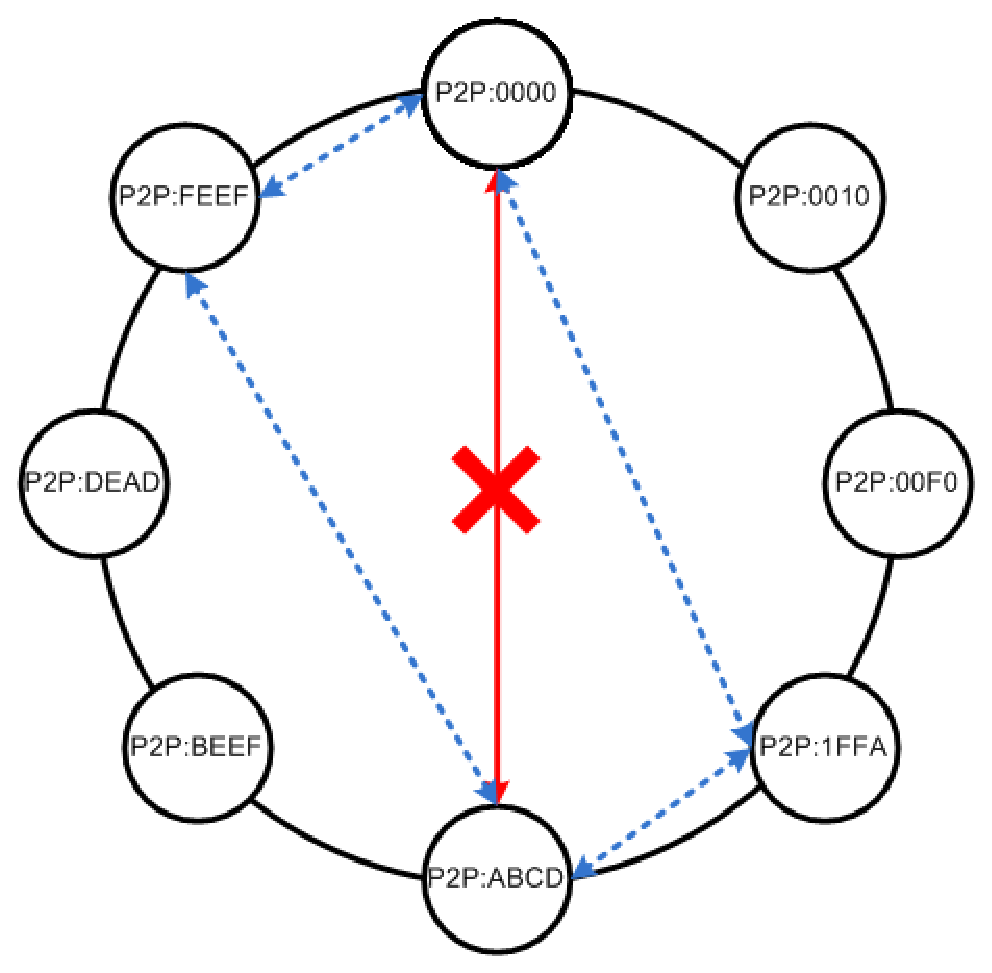
\epsfig{file=figs/relay.png.eps, width=4in}
\caption[Motivation for relays]{Creating relays across the node address space,
when direct connectivity is not possible.  Two members, 0000 and ABCD,  desire
a direct connection but are unable to directly connect, perhaps due to NATs or
firewalls.  They exchange neighbor information through the overlay and connect
to one of each other's neighbors, creating an overlap.  The overlap then
becomes a relay path (represented by dashed lines), improving performance over
routing across the entire overlay.}
\label{fig:relay}
\end{figure}

Additionally, I have added the feature to exchange arbitrary information along
with the neighbor list.  Thus far, I have implemented systems that pass
information about node stability (measured by the age of a connection) and
proximity (based upon ping latency to neighbors).  Furthermore, when overlap
changes, another mechanism can determine which subset of the peers to use; for
example, a peer may only route through the fastest or more stable overlap in
the set.

To verify the usefulness of two-hop over overlay routing, I performed
experiments and share the results in Section~\ref{relay_motivation}.  In a live
system, I have verified the accuracy and usefulness of the latency-based relay
selection algorithm in Section~\ref{relay_eval}.

\subsection{Motivation for Relays in the Overlay}
\label{relay_motivation}

The purpose of this experiment is to quantify the performance benefits of
autonomic relays.  For this experiment I used the MIT King data
set~\cite{king_data}, which contains all-to-all latencies between 1,740
well-distributed Internet hosts.  Various sizes of networks up to 1,740 nodes
were evaluated 100 times each.  The experiments were executed by running the
Brunet in simulated mode.  Once at steady state, I then calculated the average
all-to-all latency for all messages that would have taken two overlay hops or
more, the average of the low latency relay model, and the average of single hop
communication.  In the low latency relay model, each destination node form a
connection to the source node's physically closest peer as determined via
latency (in a live system by application level ping).  Then this pathway is
used as a two-hop relay between source and node.  I only look at two overlay
hops and more, as a single hop would not necessarily benefit from the work and
would be the cause of a triangular inequality.  

\begin{figure}
\centering
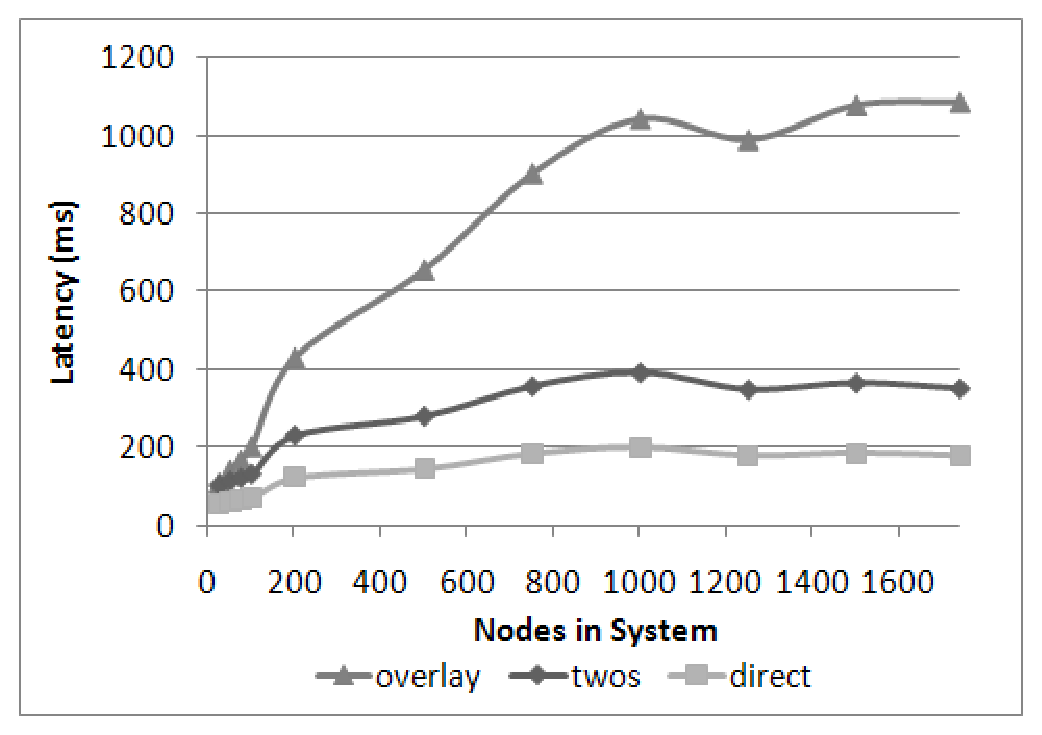
\epsfig{file=figs/relay_motivation.png.eps, width=4in}
\caption[Motivation for relays]{A comparison of the average all-to-all overlay
routing, two-hop relay, and direct connection latency in a Structured P2P
environment, Brunet, using the King data set.}
\label{fig:simulated_relays}
\end{figure}

The results are presented in Figure~\ref{fig:simulated_relays}.  The initial
starting size for the network was set to 25, because network sizes around 20
and under tend to be fully connected due to the connectivity requirements of
the system.  It is not until the network size expands past 100 and towards 200
nodes that relays become significantly beneficial.  At 100 nodes, there is
approximately a 54\% performance increase, whereas at 200 there is an 87\%
increase and it appears to grow proportionately to the size of the pool.  The
key take away is that latency-bound applications using a reasonably sized
overlay would significantly benefit from the use of two-hop relays.

\subsection{Comparing Relay Selection}
\label{relay_eval}

In this experiment, I share my experiences of testing the use of latency-aware
relays using the public P2P pool running on Planet-Lab as well as Hamachi-Free
and Hamachi-Pro relays.  Due to Hamachi not supporting relays in Linux, this
experiment was performed in Windows Vista 64-bit.  Hamachi is discussed in
greater depth in Chapter~\ref{chap:vpns}.  The testing platform consists of two
virtual machine located on the same host with a firewall preventing them from
establishing direct connections.  All experiments were repeated 5 times using a
clean configuration each time.  In Hamachi, this meant that the server would
need to re-evaluate NAT traversing capabilities and the optimal relay to use.
In Brunet, this meant a new node ID and establishing relays with peers in
different regions of the overlay.  The results are presented in
Table~\ref{tab:relay_eval}.

\begin{table}
\caption[Relay comparison]{Results of the evaluation comparing latency and
bandwidth of Hamachi relays and IPOP latency-aware autonomic relay selection.}

\centering
\begin{tabular*}{\textwidth}{@{\extracolsep{\fill}}
l
S[table-format=2.1,table-number-alignment=right]
S[table-format=2.2,table-number-alignment=right]
S[table-format=4.1,table-number-alignment=right]
S[table-format=4.2,table-number-alignment=right]
@{}
}

\hline &
\multicolumn{2}{c}{Latency} &
\multicolumn{2}{c}{Bandwidth}

\\ \hline &
\multicolumn{1}{c}{(ms)} &
\multicolumn{1}{c}{stdev} &
\multicolumn{1}{c}{Kbit/s} &
\multicolumn{1}{c}{stdev} \\ \hline
Hamachi-Free & 60.8 & 2.54 & 40.2 & 0.87 \\ \hline
Hamachi-Pro & 60.2 & 1.68 & 1000 & 1.29 \\ \hline
Latency-aware & 58.1 & 35.5 & 2245 & 1080 \\ \hline
\end{tabular*}
\label{tab:relay_eval}
\end{table}

As Hamachi was started and figured out that NAT traversal was not possible, it
began using multiple different relays as evident by several different ping
times.  Eventually Hamachi settled on a relay server and it appeared to be the
same one every time, for both Hamachi-Free and Hamachi-Pro.  The only
difference between Hamachi-Pro and Hamachi-Free is that in Pro there is a
bandwidth cap of approximately 1 Mbit/s whereas Free is limited to 40 Kbit/s.

Brunet has nodes both on Planet-Lab but also dedicated systems for
Archer~\cite{archer}.  These machines are at Universities and thus have a high
bandwidth and low latency connection to the testing site.  As witnessed by the
results, it appears that in most if not all these experiments peers had a low
latency connection to a University compute resource and it was chosen ahead of
Planet-Lab.

The two take aways are the benefit of being able to dynamically deploy relay
servers and reuse compute nodes as relay systems.  As the network grows, there
may be need to implement some form of bandwidth limit at relay nodes.

\section{Policies for Establishing Direct Connections}

Routing through a ring-structured overlay using a greedy routing algorithm
takes $log(N)$ time and adds $log(N)$ overall bandwidth for a single message.
Therefore, sending messages frequently between two peers through the overlay is
not cost effective.  What is not apparent through the algorithmic complexity
analysis is the fact that many paths in an overlay can be inefficient due to
peers routing through distant parts of the world or having limited bandwidth.
Less frequently, packets routed via the overlay can just disappear due to nodes
disconnecting or packet drops across the Internet.  To address this, Ganguly et
al.~\cite{wow} made a system for creating adaptive shortcuts.

Adaptive shortcuts enable peers to establish direct links with each other using
Brunet's builtin NAT traversal capabilities.  The approach taken by Ganguly et
al. was to monitor incoming packets from remote peers and after a certain
threshold was passed the system automatically makes a direct connection to the
remote peer.  As a result of this transparency, software using the overlay
could simply start this service without making any additional changes to the
application.  

\subsection{Limitations}

Unfortunately this approach comes with limitations.  There was never any
systematic understanding of behaviors that should signify the creation of a
direct link or when a direct link should be closed.  Thus applying the layer
naively could result in connection churn, which would have ramification on the
routability of the network.  Thus a compromise was made to have it enabled only
for selected traffic, which in the case as described by Ganguly et
al.~\cite{wow} was IP or VN traffic.

Two issues made the approach no longer feasible:  the increase in size of the
overlay network and the securing of IP links.  The Internet drops packets at
approximately .00835\% of the time according to the data provided by
iPlane~\cite{iplane}.  This compounded with the fact that an overlay message
may take $log(N)$ hops significantly increases the likelihood of a packet
dropping before arriving at its destination.  Adding a security model makes
this even more complicated, because a trusted link must be established before
routing any messages between the end points.  In the case of DTLS, this can
result in 6 messages traversing the overlay~\ref{fig:dtls}, prior to the first
IP packet.  If peers must first establish a trusted link and then transmit a
certain amount of packets in a given time, there is a reasonable chance that
they may never naturally trigger the creation of an adaptive link.

In practice, it was quite common for this not to succeed and, in fact, security
links were often times not even formed.  To verify this, I implemented a
network profiling tool and deployed it on to PlanetLab.  The monitoring tool
measured the delay and success of sending messages between the node and every
other node in the overlay.  The drop rate and latency for a round trip message
per hop distance between two peers are presented in
Figure~\ref{fig:drop_rate_plab} and Figure~\ref{fig:latency_plab},
respectively.  The data in those figures is compared to data retrieved from
iPlane, which makes it clear that PlanetLab exacerbates the situation.  While
this is a well-known issue, it is a very important conclusion since many of the
public systems provided by my research group rely on PlanetLab.

\begin{figure}[ht]
\centering
\includegraphics[width=3.5in]{figs/latency_plab.eps}
\caption[Latency in PlanetLab deployment]{Average latency in a round trip
message between two nodes specified by the amount of hops between them.  The
PlanetLab average is compared against data available from iPlane.  The CDF for
node distance is also plotted for reference.}
\label{fig:latency_plab}
\end{figure}

\begin{figure}[ht]
\centering
\includegraphics[width=3.5in]{figs/drop_rate.eps}
\caption[Drop rate in PlanetLab deployment]{Average drop rate in a round trip
message between two nodes specified by the amount of hops between them.  The
PlanetLab average is compared against data available from iPlane.  The CDF for
node distance is also plotted for reference.}
\label{fig:drop_rate_plab}
\end{figure}

\subsection{On-Demand Connections}

Before defining a new architecture, I measured the network traffic of active
and idle applications that were of interest to typical P2P VPNs,
Condor~\cite{condor0} and data transfers.  Data transfers tend to be simple, if
they are TCP driven, first a TCP link must be established, then data
transferred, and finally the link is closed.  Condor is a job schedule
management tool, which is discussed in more depth in
Chapter~\ref{chap:gridappliance}.  The important aspect for this section is
understanding that all nodes in a Condor pool have a relationship with a
manager node.  Their behavior is to initially send a registration message
containing the details of the node and thereafter to send a one-way message
stating their presence every 5 minutes or so.

The next step was determining the cost of creating a connection versus routing
via the overlay.  This cost needs to consider that before a single IP packet
can be routed, a security link must be established.  In Brunet, the creation of
a link requires 1 round trip message across the overlay, whereas the security
link, as mention earlier, takes 3.  So it is intuitive that sending a single
packet secured through an end-to-end channel via a direct link is far more
efficient than doing so via the overlay.  So instead of having a meter
determining when to create connections, connections should be made as soon as
there is interest in communication, in other words, ``on-demand.''  In a DHT
system, this may be done prior to sending or retrieving data from the DHT.  In
a VPN, this may be during the mapping of IP to P2P as described in
Section~\ref{vpns:arp}, which occurs before secure link establishment.
Unfortunately, this has the side affect of not being transparent to
applications using the P2P software's interface at the cost of being more
responsive.

The creation of on-demand connections results in a higher frequency of
connection establishment.  As a result, better heuristics are necessary in
order to determine when to close unused connections.  Using the profiling
information retrieved before with regards to Condor's one-way ``heartbeat''
messages, it was important that a connection was only closed if it was unused
in both directions.  Otherwise the manager would be constantly closing
connections and peers would randomly disappear from Condor for periods of time.
An algorithm that seems to have worked so far is based upon something I call a
time-based cache.  Initially, entries are stored in a hashtable; after a
certain period of time, they are moved to a second hashtable, and those in the
second hashtable are lost.  If an entry is accessed while in the second
hashtable or not at all, it is added to the first hashtable and if applicable
removed from the second hashtable.  When an entry is removed from the cache, it
causes an eviction notice, which results in the connection being removed.  The
timer is based upon a 7.5 minute timer, so that an inactive connection will be
closed within 7.5 to 15 minutes.

The applicability of on-demand connections compared to Chota was evaluated
using the simulator with 1,024 nodes and a drop rate of 0.00925\% as found on
PlanetLab.  The On-demand connections were established using the exact semantics
of the On-demand protocol; however, the behavior of establishing Chota
connections is a little complicated, since the traffic behavior of successful
and unsuccessful connection attempts is not identical.  To address this, I
simulated an ideal Chota situation:  the nodes optionally establish a security
connection via the overlay, then they exchange a round trip message, and
finally establish a direct connection between each other.  The On-demand
approach involved optionally creating a security connection followed by the
direct connection.  

\begin{figure}[ht]
\centering
\includegraphics[width=3.5in]{figs/connections.eps}
\caption[Time to form a direct connection]{CDF of the connection establishment
time for secure and security-free Chota and On-demand connections in an overlay
of 1,024 nodes and a drop rate of .00925\%.}
\label{fig:connections}
\end{figure}

While this evaluation model creates a highly ideal situation for Chota
etablishment.  The results in Figure~\ref{fig:connections} make it clear that
Chota is not ideal for this type of application and that security only makes
the issues worse.  The On-demand connections show a significant improvement, but
there still exists an obvious issue with connection establishment that will
only be made worse as the system expands.  Perhaps using multiple paths on the
overlay can improve this situation packet drops on the overlay may have high
correlation rather than being uniformly random.

In application, this modification made the Archer, which uses both secure links
and Condor, significantly more stable.  As the system expanded, nodes were
constantly appearing and disappearing, users jobs were being lost due to
disconnectivities, and users were complaining about being unable to even submit
jobs into the system.  Since the change, the issues have been resolved.

\section{Broadcasting IP Broadcast and Multicast Packets Via the Overlay}

The use of a private virtual overlay enables a new method for sending multicast
and broadcast packets. In the original approach to IPOP, broadcasting a packet
to the entire overlay  is not suitable because the overlay could consist of
peers from other VPNs and those not even involved with VPN operations, while
approaches that generate unicast messages when a broadcast or multicast packet
arrives at the VPN (e.g. by querying a DHT key where all peers in the VPN would
place their overlay address so that they could receive the packets) do not
scale well. The abstraction of a private virtual overlay enables scalable
broadcasting within a VPN because the only peers in the private overlay are
peers for a single VPN.  Like the broadcast revocation discussed earlier, IP
broadcasting and multicasting use the method described in
Appendix~\ref{broadcast} to efficiently distribute messages.  Though in VPN
situations, many peers may already have connections to most if not all of their
VPN peers, thus the broadcast algorithm has been modified to allow a peer to
select how many peers they would like to forward the message to.  Otherwise in
many cases, this algorithm will degenerate into one similar to the previous
approach.  

\begin{figure}
\centering
\caption{IP Broadcast using the DHT compared to overlay broadcast}
\label{fig:ipbroadcast}
\end{figure}

A validation of the overlay broadcast method for IP broadcast and multicast
communication comparing it to the original DHT method is presented in
Figure~\ref{fig:ipbroadcast}.  Metrics measured include bandwidth used by the
packet originator and time required for all peers to receive the packet.
System bandwidth remains the same as bounded-broadcast requires exactly $N$
messages to broadcast the message to the entire overlay.  By using a broadcast
algorithm to route multicast and broadcast IP packets instead of the unicast
packets, the sending node has much less used bandwidth.  The time required by
the DHT approach involves the time to retrieve all entries from the DHT and the
latency to the peer farthest away.  Whereas the broadcast approach has no DHT
lookup and is somewhere around the average latency in the system multiplied by
$\log^2(N)$.

\section{Full Tunnel VPN Operations}
\label{full_tunnel}

The configuration detailed so far describes a split tunnel: a VPN connection
that handles \emph{internal VPN traffic only, not Internet traffic}.  Prior to
this work, only centralized VPNs currently support full tunnel: providing the
features of a split tunnel in addition to securely forwarding \emph{all their
Internet traffic} through a VPN gateway.  A full tunnel provides network-layer
privacy when a user is in a remote, insecure location such as an open wireless
network at a coffee shop by securely relaying all Internet traffic through a
trusted third party, the VPN gateway.  Both models are illustrated in
Figure~\ref{fig:tunnel}.

\begin{figure}
\centering
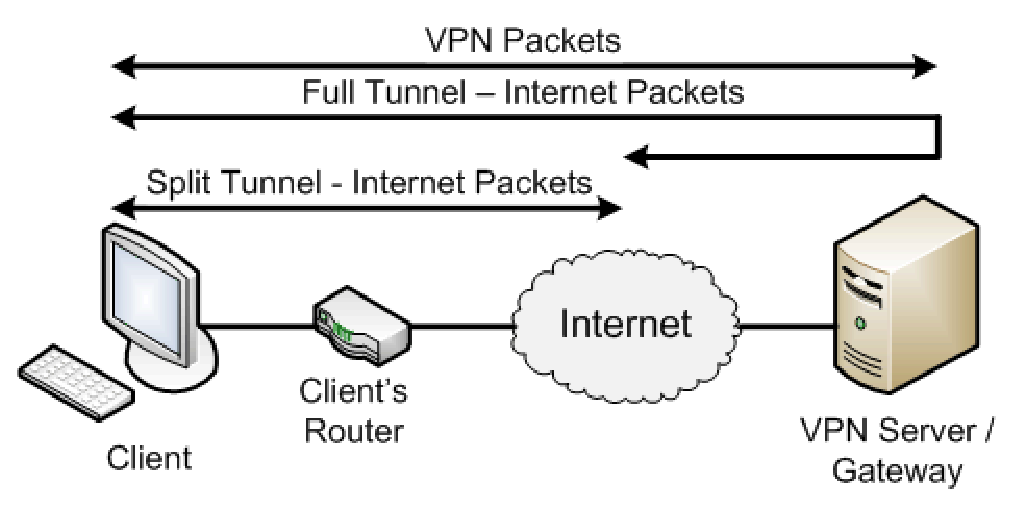
\epsfig{file=figs/tunnel.png.eps, width=4in}
\caption[An example of both full and split tunnel VPN modes]{An example of both
full and split tunnel VPN modes.  In both, packets for the server are sent
directly to the server.  In split tunnel mode, Internet packets bypass the VPN
and are routed directly to the Internet.  In full tunnel mode, Internet packets
are first routed to the VPN gateway, and then to their Internet destination.}
\label{fig:tunnel}
\end{figure}

Central VPN clients use full tunneling through a routing rule swap, setting the
default gateway to be an endpoint in the VPN subnet and traffic for the VPN
server is routed explicitly to the LAN gateway.  This rule swap causes all
Internet packets to be routed to the VN device and the VPN software can then
send them to the remote VPN gateway.  At the VPN gateway, the packet is
decrypted and delivered to the Internet.  A P2P system encounters two
challenges in supporting full tunnels:  1) P2P traffic must not be routed to
the VPN gateway and 2) there may be more than one VPN gateway.  I address these
issues and provide a solution to this problem in Section~\ref{full_tunnel}.

The challenges faced in a decentralized P2P VPN are providing decentralized
discovery of a VPN gateway and supporting full tunnel mode in a P2P environment
such that all P2P traffic is sent to the intended receiver directly instead of
through the gateway.  The remainder of this section covers gateway and
client solutions to address these challenges.

\subsection{The Gateway}
\label{the_gateway}
A gateway can be configured through NAT software, like masquerading in IPtables
or Internet Connection Sharing with Windows.  This automatically handles the
forwarding of packets received on the NAT interface to another interface
bringing the packet closer to its destination.  Similarly, incoming packets
on the outgoing interface must be parsed in order to determine the destination
NAT client.

Following from the original design of the VPN state machine in
Figure~\ref{fig:vn}, if a VPN is a gateway, the VPN state machine no longer
rejects packets, when the destination is not in the VPN subnet, though when the
VPN gateway mode is disabled these packets are still rejected.  When enabled,
all Internet and non-VPN based traffic is written to the TAP device setting the
destination Ethernet address to the TAP device.  The remaining configuration is
identical to other members of the system as packets from the Internet will
automatically have the clients IP as the destination as a product of the NAT.
To provide for dynamic, self-configuring systems, VPN gateways announce their
availability via an entry in the DHT.  As future work, this approach can be
explored to provide intelligent selection and load balancing of gateways.

\subsection{The Client}
VPN Clients wishing to use full tunnel must redirect their default traffic to
their VN device.  In the prototype VPN model, a virtual IP address is allocated
for the purpose of providing distributed VN services DHCP and DNS.  This same
address is used as the the default gateway's IP.  Because this IP address never
appears in a Internet bound packet, only its Ethernet address does, as shown in
Figure~\ref{fig:tunnel_packet}, this approach enables the use of any and
multiple remote gateways.

\begin{figure}
\centering
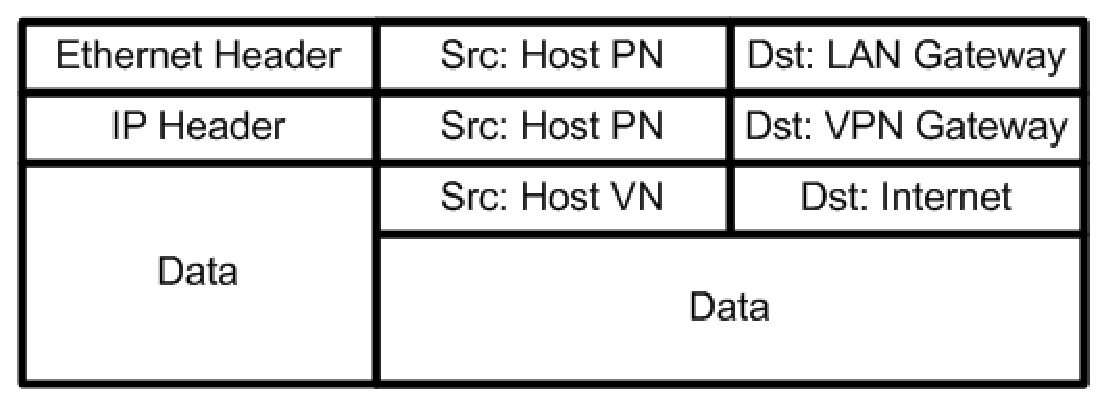
\epsfig{file=figs/tunnel_packet.png.eps, width=4in}
\caption[The contents of a full tunnel Ethernet packet]{The contents of a full
tunnel Ethernet packet.  PN and VN are defined as physical and virtual network,
respectively.}
\label{fig:tunnel_packet}
\end{figure}

To support full tunnel mode, the VPN's state machine has to be slightly modified
to handle outgoing packets destined for IP addresses outside of the VPN, only
rejecting them when full tunnel client mode is disabled.  When enabled, the VPN
software sends packets to the remote peer acting as a full tunnel gateway.
Likewise, incoming packets that have a source address outside the subnet should
not be rejected but instead the overlay address should be a certified VPN
gateway prior to forwarding the packet.

To select a remote gateway, peers query the DHT.  As there may be multiple
gateways in the system, the peer randomly selects one, forwarding packets to
that node.  To ensure reliability, when the client has not heard from the
gateway recently, the client sends a liveness query to the gateway.  If the
gateway is down, the taken pessimistic approach finds a new gateway when
the next Internet packet arrives.

The real challenge in applying full tunnel VPN mode to P2P VPNs is the nature
of the P2P system, namely dynamic connections.  Peers do not know ahead of time
what remote peer connections will be thus a simple rule switch does not work.
The original approach was to watch incoming connection requests and adding
additional routing rules on demand, though this is only reasonably feasible
with UDP as a TCP handshake message would need to be intercepted and potentially
replayed by the local host in order to enable the rule and allow proper routing.
The real drawback of the approach though is that UDP messages can easily be
spoofed by remote peers enabling unsecured Internet packets to be leaked in the
public environment.  Even if the connections are secured, it could take some
time for the peers to recognize a false connection attempt and delete the rule.

A solution to the security problem is to have all traffic directly routed to
the VN device with no additional routing rules.  The VN is then responsible for
filtering P2P traffic and forwarding it to the LAN's gateway via Ethernet
packets.  In the VPN application, outgoing IP packets' source ports are
compared to VPN application's source ports.  Upon a match, the VPN application
directs the packet to the LAN's gateway.  The three steps involved in this
process are 1) translating the source IP address to match the physical
Ethernet's IP address, 2) encapsulating the IP packet in an Ethernet packet
with a randomly source address~\cite{sc09} and the destination the LAN's
gateway, and 3) sending the packet via the physical Ethernet device.  Sending
an Ethernet packet is not trivial as Windows lacks support for this operation
and most Unix systems require administrator privilege.  An alternative, platform
independent solution uses a second TAP device bridged to the physical Ethernet
device, allowing Ethernet packets to be sent indirectly through the Ethernet
device via the TAP device.  Because the solution results in incoming packets to
arrive at a different IP address than the actual original source IP address TCP
does not work in this solution.  This method has been verified to work on both
Linux and Windows using OS dependent TAP devices and bridge utilities.

\subsection{Full Tunnel Overhead}
\label{full_tunnel_eval}

While the full tunnel client method effectively resolves the lingering problem
of ensuring that all packets in a full tunnel will be secure, it raises an
issue:  could the effect of having all packets traverse the VPN application be
prohibitively expensive.  Analysis of this approach compares it with one that
uses the traditional routing rule switch.  Figure~\ref{tab:full_tunnel_eval}
present the ping time from a residential location to one of Google's IP
addresses using a gateway located at the University of Florida when the VPN is
in split tunnel mode, full tunnel using the routing rule switch, and full
tunnel using Ethernet forwarding.  The results express that there is negligible
difference between the full tunnel approaches.  One interesting result is the
latency to gateways public address in the routing test, which most likely is a
result of the ping being sent insecurely avoiding the VPN stack completely.

\begin{center}
\begin{table}
\caption[Full tunnel evaluation]{Latency results comparing full tunnel
approaches measured in ms.  Legend: GW Pri - gateway's VPN address, GW Pub -
gateway's VPN address, Ethernet - full tunnel Ethernet packet method, Routing -
full tunnel routing rule switch, None - split tunnel or no VPN.}
\begin{tabular*}{\textwidth}{@{\extracolsep{\fill}}
l
S[table-format=2.1,table-number-alignment=right]
S[table-format=2.1,table-number-alignment=right]
S[table-format=2.1,table-number-alignment=right]
@{}
}

\hline &
\multicolumn{1}{c}{Google} &
\multicolumn{1}{c}{GW Pri} &
\multicolumn{1}{c}{GW Pub} \\ \hline \hline
Ethernet & 70.6 & 12.9 & 13.9 \\ \hline
Routing & 71.4 & 13.2 & 11.0 \\ \hline
None & 66.1 & N/A & 10.9 \\ \hline
\end{tabular*}
\label{tab:full_tunnel_eval}
\end{table}
\end{center}
